\begin{frame}
  \frametitle{Ingresos tributarios del GNC}
  \vspace{0.05cm}
  {\centering\small\color{blue!70!black}Fuente: MHCP y cálculos propios\par}
  \vspace{-0.1cm}
  \begin{center}
    \scalebox{0.70}{
      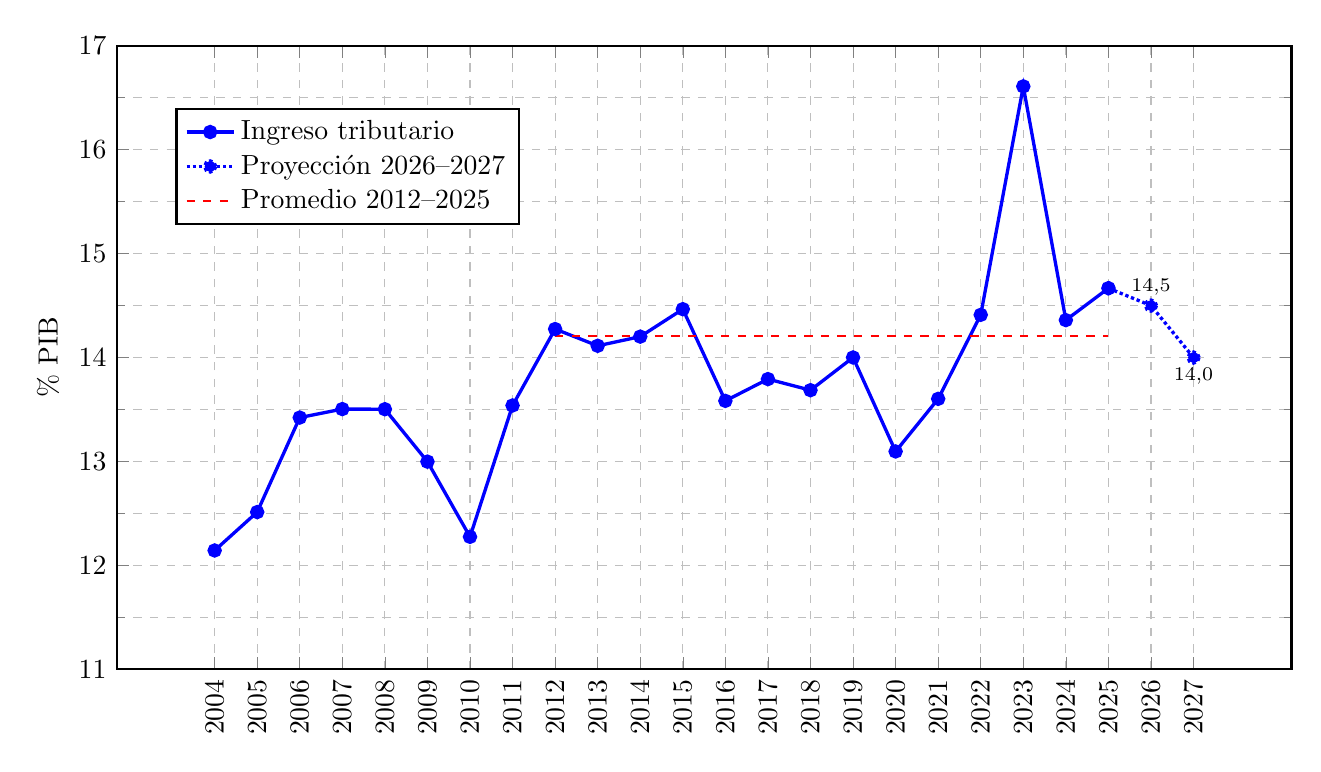
\begin{tikzpicture}
      \begin{axis}[
          width=16.5cm,
          height=9.5cm,
          ylabel={\% PIB},
          xtick={1,...,24},
          xticklabels={2004,2005,2006,2007,2008,2009,2010,2011,2012,2013,2014,2015,2016,2017,2018,2019,2020,2021,2022,2023,2024,2025,2026,2027},
          x tick label style={rotate=90, anchor=east},
          ymin=11,
          ymax=17,
          grid=major,
          grid=both,
          grid style=dashed,
          minor y tick num=1,
          legend style={at={(0.05,0.9)}, anchor=north west},
          legend cell align={left},
          thick
      ]

%      % Ingreso Total
%      \addplot[
%          mark=square*,
%          dashed,
%          red
%      ] coordinates {
%          (1,13.2) (2,13.6) (3,14.8) (4,15.1) (5,15.8) (6,15.4) (7,13.8)
%          (8,15.2) (9,16.1) (10,16.8) (11,16.5) (12,16.1) (13,14.9) (14,15.7)
%          (15,15.1) (16,16.2) (17,15.3) (18,16.1) (19,16.2) (20,18.7) (21,16.5) (22,16.3)
%      };

      % Ingreso Tributario
      \addplot[
          mark=*,
          very thick,
          blue
      ] coordinates {
          (1,12.143374781333) (2,12.512922935182) (3,13.422519626341)
          (4,13.504136808694) (5,13.502896432021) (6,12.998278577445)
          (7,12.274640215080) (8,13.538733320074) (9,14.274306787792)
          (10,14.112999163893) (11,14.201344469556) (12,14.465553461687)
          (13,13.583123624578) (14,13.792707184015) (15,13.685807298757)
          (16,14.000802323615) (17,13.096318634224) (18,13.602505788695)
          (19,14.411093615786) (20,16.609633331004) (21,14.360250034683)
          (22,14.667199811906)
      };

      % Proyección MHCP 2026--2027, hoja 1.3 de Figuras.xlsx
      \addplot[
          color=blue,
          mark=*,
          very thick,
          densely dotted
      ] coordinates {
          (22,14.667199811906) (23,14.5) (24,14.0)
      };

      \node[anchor=south] at (axis cs:23,14.5) {\scriptsize 14,5};
      \node[anchor=north] at (axis cs:24,14.0) {\scriptsize 14,0};

      % Promedio 2012--2025 (Ingreso Tributario)
      \pgfmathsetmacro{\avgtrib}{14.204546109299}
      \addplot[
          red,
          dashed,
          thick
      ] coordinates {(9,\avgtrib) (22,\avgtrib)};

      \legend{Ingreso tributario, Proyección 2026--2027, Promedio 2012--2025}
      \end{axis}
      \end{tikzpicture}
    }
  \end{center}
  \note{[Sources] Figuras.xlsx, hoja 1.3, B1:Y1 y B3:Y4, versión del 17 de septiembre de 2026. Fuente indicada en el Excel: MHCP. Ingreso tributario del GNC, 2004--2027, en porcentaje del PIB. Las proyecciones para 2026 y 2027 son 14,5\% y 14,0\% del PIB, respectivamente. La línea discontinua conecta las proyecciones con el dato de 2025. Promedio aritmético de 2012--2025, calculado con los valores sin redondear de J3:W3: 14,204546109299\% del PIB.}
\end{frame}
